\section{主机环境}
\begin{itemize}
\item \textbf{创建分区}:在与Host相同的硬盘上创建或者单独一块硬盘的分区创建.

\item \textbf{创建路径}:在分区上创建必要的路径并设置好权限.

\item \textbf{下载源码包}.

\item \textbf{创建专用账户}:并为之设置好相应环境.

\item \textbf{搭建主机编译环境}:在Ubuntu中,用以下命令即可完成\\
\shell{sudo apt-get install build-essential}\\
最后确认以下几条:
\begin{itemize}
\item  使用的是bash: ``\texttt{echo \$0}"或``\texttt{env | grep SHELL}"

\item sh是指向bash符号链接:在/bin目录下查看.

\item /usr/bin/awk是指向/usr/bin/gawk的符号链接:若不是则创建\\
\shell{sudo ln -sv gawk awk}

\item /usr/bin/yacc是指向/usr/bin/bison的符号链接:在Ubuntu中,需要另外
安装bison.

\end{itemize}

\end{itemize}

\section{编译工具链}
编译过程中,注意检查几个关键包是否正常,例如gcc.

\section{编译基本系统}
利用之前编译好的工具链来编译出基本的系统,进入chroot环境后,利用PATH设置
搜索顺序,新编译的工具逐渐取代工具链中的工具,直到最后编译完成.此时,我们
不再需要工具链了,可以将其删除或者保存以便以后继续编译系统使用.然后重新进入
chroot环境.以后每次重新进入Host开始编译基本系统工作时,将要做的操作保存成脚本,每次运行一下即可:
\begin{verbatim}
#!/bin/bash
#readForLFS.sh

export LFS=/mnt/lfs

mount -v --bind /dev $LFS/dev
mount -vt devpts devpts $LFS/dev/pts -o gid=5,mode=620
mount -vt proc proc $LFS/proc
mount -vt sysfs sysfs $LFS/sys
mount -vt tmpfs tmpfs $LFS/run

chroot "$LFS" /usr/bin/env -i \
    HOME=/root TERM="$TERM"   \
    PS1='\u:\w\$ '            \
    PATH=/bin:/usr/bin:/sbin:/usr/sbin \
    /bin/bash --login
\end{verbatim}

\section{配置系统}
包括配置主机信息、网络环境等等,值得注意的是,完成/etc/sysconfig/console的配置时,
只需要指定UNICODE和LEGACY\_CHARSET值,其余用默认值即可.

\section{内核编译}
第一次解压准备编译前,先做一下清理:\\
\shell{make mrproper}\par
以后编译前清理使用命令:\\
\shell{make clean}\par
用图像界面选择内核功能:\\
\shell{make menuconfig}\par
编译:\\
\shell{make}\par
安装模块:\\
\shell{make modules\_install}\par
接下来复制编译好的内核等.
\par
其中,关键的一步就是选择内核的功能,由于我使用VMware来完成的,未正确选择驱动
功能,导致每次启动LFS遇到错误:``end kernel panic - not syncing: VFS: Unable to
 mount root fs on unknown - block(0,0)".这里需要针对VMware选择的模块是:``Device Drivers"$\rightarrow$``Fusion MPT device support"菜单下的功能选择将
 其编译进内核.另外还有网卡模块:``Device Drivers"$\rightarrow$``Networking support"$\rightarrow$``Ethernet (10 or 100Mbit)"$\rightarrow$``AMD PCnet32 PCI support"\footnote[1]{直接搜索关键字``ethernet"即可找到在菜单中的位置}.另外,文件系统可以添加对NTFS格式的支持等等,具体见《鸟哥-基础篇》和``有道笔记".
 
 \section{配置grub} 
 对grub的详解见《鸟哥-基础篇》.
 \subsection{/boot在/dev/sda2}
 此时并不需要重新安装grub,只需要修改Host的/boot/grub/grub.cfg文件,添加一条
 引导LFS的菜单:
 \begin{verbatim}
 menuentry "LFS" {
    insmod ext2
    set root=(hd0,2) #第一块硬盘的第二个分区
    linux /boot/vmlinuz-3.16.2-lfs-7.6 root=/dev/sda2 ro
 }
\end{verbatim}
\vspace{-2ex}
 \par
 另外/etc/fstab中根目录的挂载是:\\
\verb" /dev/sda2  /   ext4    defaults    0   1"

\subsection{/boot在/dev/sdb1}
\subsubsection{保留Host}
此时也不需要重新安装grub,只需要修改Host的/boot/grub/grub.cfg文件,添加一条
 引导LFS的菜单:
 \vspace{-1ex}
 \begin{verbatim}
 menuentry "LFS" {
    insmod ext2
    set root=(hd1,1) #第二块硬盘的第一个分区
    linux /boot/vmlinuz-3.16.2-lfs-7.6 root=/dev/sdb1 ro
 }
\end{verbatim}
\vspace{-2ex}
 \par
 另外/etc/fstab中根目录的挂载是:\\
\verb" /dev/sdb1  /   ext4    defaults    0   1"

\subsubsection{不保留Host}
安装grub:\\
\shell{grub-install --force /dev/sdb}\footnote[1]{不加``--force"会报错}
\par
修改LFS系统/boot/grub/grub.cfg,添加引导LFS的菜单:
\vspace{-1ex}
 \begin{verbatim}
 menuentry "LFS" {
    insmod ext2
    set root=(hd0,1) #第一块硬盘的第一个分区
    linux /boot/vmlinuz-3.16.2-lfs-7.6 root=/dev/sda1 ro
 }
\end{verbatim}
\vspace{-2ex}
 \par
 另外/etc/fstab中根目录的挂载是:\\
\verb" /dev/sda1  /   ext4    defaults    0   1"
\par
然后移除原Host所在硬盘,并设置LFS所在硬盘为第一块硬盘.
\begin{figure}[h]
\centering
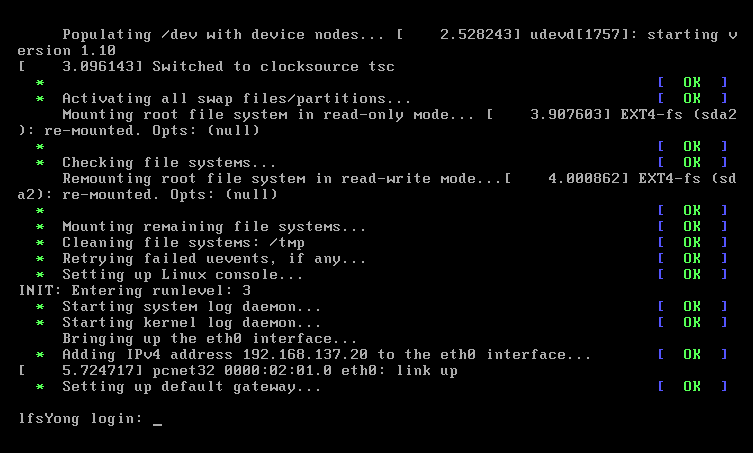
\includegraphics[width=\textwidth]{pic/LFS.PNG}
\caption{LFS启动成功}
\end{figure}

